\title{Template}
\author{Robert Poenaru
}
\date{\today}
\documentclass[11pt]{article}
%\documentclass{acmconf}

\usepackage[paper=a4paper,dvips,top=1.5cm,left=1.5cm,right=1.5cm,
    foot=1cm,bottom=1.5cm]{geometry}

\usepackage{times}
\usepackage{graphicx}
\usepackage[fleqn]{amsmath}
\usepackage{amsfonts}
\usepackage{amssymb}
\usepackage{amsthm}
\usepackage{amsopn}
\usepackage{xspace}
\usepackage{array}
\usepackage{epsfig}
\usepackage{lipsum}
\usepackage{tikz}
\usepackage{pgfplots}
\begin{document}

\maketitle
\section{Plot}
\subsection{As a pdf}
This is a plot inside a latex document as a pdf file.
\begin{figure}[h]
    \centering
    \includegraphics[scale=0.6]{../errorPlots/multiple.pdf}
    \caption{The plot as a \texttt{.pdf} file.}
\end{figure}
\subsection{As latex plot - using \texttt{tikz}}

\begin{tikzpicture}
\begin{axis}
\addplot[color=red]{exp(x)};
\end{axis}
\end{tikzpicture}
%Here ends the furst plot
\hskip 5pt
%Here begins the 3d plot
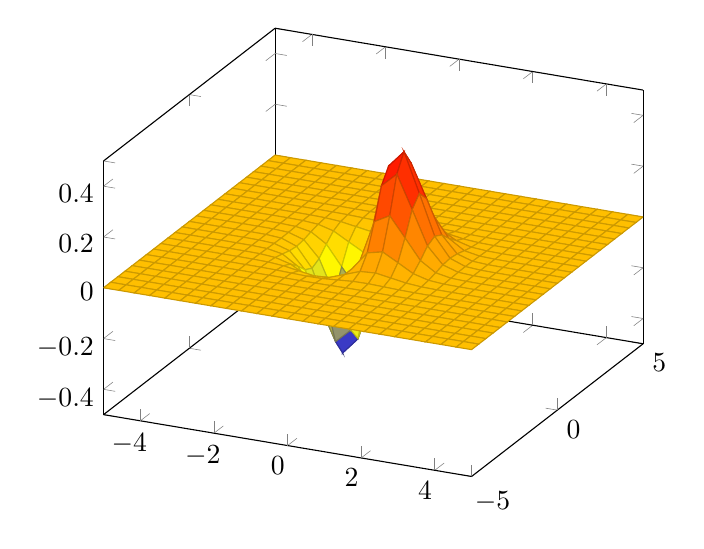
\begin{tikzpicture}
\begin{axis}
\addplot3[
    surf,
]
{exp(-x^2-y^2)*x};
\end{axis}
\end{tikzpicture}

\end{document}